% State the application of the profile chain
% Describe the in group time measure and why it is relevant.
% Embed tables of the steady state over time
% Highlight critical points, discuss the shape of the curve?
% Mention how an invariant could be applied to adjust the schedule to improve the IGT by increasing P.
% Make a quality of service argument?

\section{Profile Chain Applications}


The DGI focuses on managing power resources in a microgrid environment.
Resources can only be managed effectively when multiple DGI coordinate together to manage those resources.
Without another DGI to coordinate with, the DGI has a limited range of options to manage power generation, storage and loads.
Therefore, the amount of time DGI will spend coordinating with another process is of particular interest.
\cite{CRITIS2012} defines an ``In Group Time'' (IGT) metric to measure the amount of time a DGI process spends coordinating with at least one other process.
In this work, we define IGT based on the steady state of the profile chain.
Let $\pi=Steady(P)$ for some profile chain.
The IGT is the sum of all states in $\pi$, save the first state where the process is alone:

\[ IGT = \sum_{i=2}^{m} \pi_i \]

The IGT is a number between 0 and 1.
It represents the probability a random observation sees a group of at least two members.
The steady state distributions are presented as stacked bar graphs in Figures \ref{fig:3process}, \ref{fig:4process}, \ref{fig:5process} and \ref{fig:6process}.
Each complete bar in the graph indicates the IGT.
The components of each bar represent the probability the system is in a specific state for a random observation of the system.
The height of the component represents the relative probability of observing that state when in a group.

\begin{figure}
    \centering
    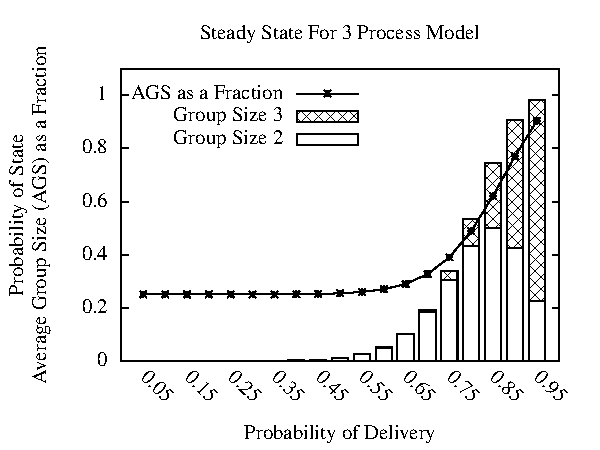
\includegraphics[width=0.65\textwidth]{ss-3process.pdf}
    \caption{Steady state distribution for 3 processes.}
    \label{fig:ss-3process}
\end{figure}

\begin{figure}
    \centering
    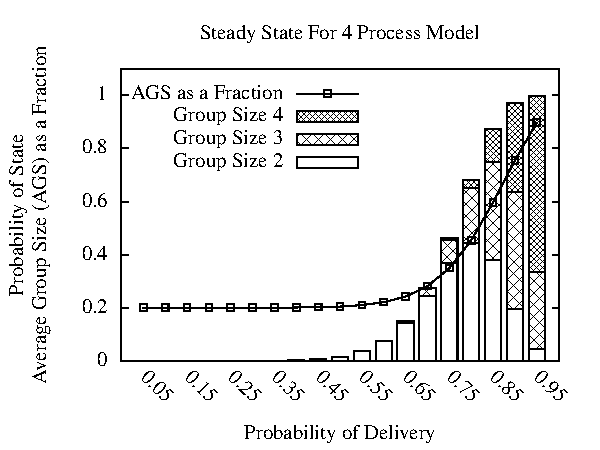
\includegraphics[width=0.65\textwidth]{ss-4process.pdf}
    \caption{Steady state distribution for 4 processes.}
    \label{fig:ss-4process}
\end{figure}

\begin{figure}
    \centering
    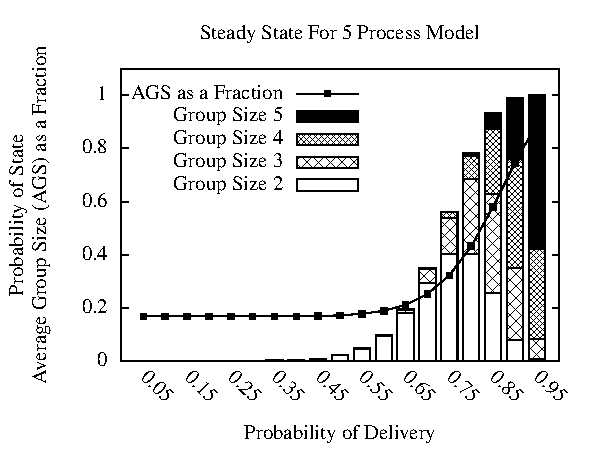
\includegraphics[width=0.65\textwidth]{ss-5process.pdf}
    \caption{Steady state distribution for 5 processes.}
    \label{fig:ss-5process}
\end{figure}

\begin{figure}
    \centering
    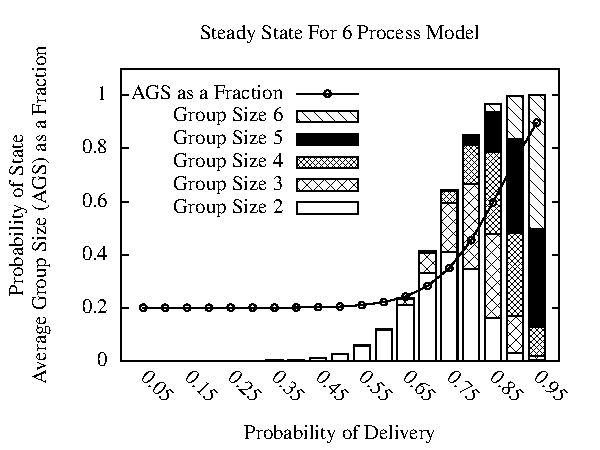
\includegraphics[width=0.65\textwidth]{ss-6process.pdf}
    \caption{Steady state distribution for 6 processes.}
    \label{fig:ss-6process}
\end{figure}

The profile chain can be used to ensure the FREEDM smart-grid is able to continue operating despite network issues.
The profile chain can be combined with different message sending strategies to maintain service.
For example, the DGI can change to a slower mode of operation to ensure operation continues normally despite connectivity issues.
By selecting different strategies depending on the message delivery probability the DGI can offer high performance in good network conditions and an acceptable level of service during faults.
